\documentclass[11pt,a4paper]{article}
\usepackage[margin=26mm]{geometry}
\usepackage[utf8]{inputenc}
\usepackage[T1]{fontenc}
\usepackage[italian]{babel}
\usepackage{amsmath,amssymb,graphicx,booktabs}
\usepackage{array,tabularx}
\usepackage[hidelinks]{hyperref}
\setlength{\emergencystretch}{2em}

\graphicspath{{images/}}

\title{SemEval 2027 Task 1}
\author{Giovanni Giuseppe Iacuzzo}
\date{\today}

\begin{document}

\maketitle

\begin{abstract}
In una conversazione, identificare il passaggio che risolve un riferimento implicito e formulare una risposta fedele a quel passaggio richiedono decisioni diverse. Studiamo se riapplicare un singolo strato di un Transformer a pesi condivisi durante l'inferenza possa migliorare una delle due decisioni a un costo sostenibile. Usiamo il subtrack 2a di RETECO per variare la profondità del riordinatore su candidati fissati e il 2b per variare quella del generatore a parità di passaggi di riferimento. Presentiamo l'implementazione e una prima misura della qualità dei candidati. Su 280 turni di validazione interna appartenenti a dieci domini, dopo un'epoca di addestramento del bi-encoder, la fusione dei ranking contestuali raggiunge una nDCG@10 macro di 0,6242, a fronte di 0,4167 per BM25 e 0,3801 per il modello denso. Il vantaggio relativo dei due retriever cambia segno tra i due gruppi di collezioni rappresentati. Queste misure caratterizzano il primo stadio del sistema. Per il riordinamento e la generazione definiamo confronti appaiati rispetto al decoder a profondità originale; la stima dell'effetto della ricorrenza resta aperta.
\end{abstract}
\noindent\textbf{Parole chiave}\quad recupero conversazionale; riordinamento neurale; generazione fondata su evidenze; profondità ricorrente; RETECO.

\section{Introduzione}
Una domanda come «E in quel caso chi può presentare ricorso?» lascia indeterminati sia il procedimento sia la persona interessata. I turni precedenti consentono di ricostruire entrambi, ma possono anche introdurre termini riferiti a casi ormai esclusi. Un sistema di recupero deve scegliere quali elementi della storia preservare nella ricerca. Una volta fornito il passaggio pertinente, il generatore affronta un secondo problema: stabilire quali condizioni riportare nella risposta e quali affermazioni l'evidenza consenta effettivamente di sostenere.

RETECO (SemEval 2027, Task~1) studia il recupero condizionato dal tempo nel Track~1, costruito su TEMPO, e dal dialogo nel Track~2, costruito su RECOR \cite{reteco,recor}. Ci concentriamo sul secondo. Nel subtrack~2a ogni turno richiede una lista ordinata di documenti del dominio. Nel~2b i passaggi pertinenti sono forniti dagli organizzatori e il sistema produce una risposta in inglese. Questa scelta sperimentale permette di attribuire un cambiamento nella risposta al generatore anche quando la ricerca sul corpus è difficile. Il caso in cui la generazione dipende dai documenti recuperati appartiene al subtrack~2c ed è esterno al presente studio.

La domanda che poniamo è operativa: una seconda applicazione dello stesso strato del decoder modifica utilmente l'ordine dei candidati o il sostegno documentale delle risposte? Il costo aggiuntivo può essere giustificato per un compito e risultare superfluo per l'altro. Nel 2a misuriamo quindi sia la disponibilità di evidenze tra i candidati sia la loro posizione dopo il riordinamento. Nel 2b valutiamo separatamente il contributo dell'adattamento supervisionato e quello della profondità a inferenza. Il primo risultato empirico riguarda la scelta dei candidati; l'efficacia del loop costituisce l'ipotesi da verificare.

\section{Stato dell'arte}

\subsection{Dal contesto conversazionale alla query di ricerca}
Nel recupero conversazionale, la pertinenza di un passaggio dipende dal significato che il turno corrente assume nel dialogo. QReCC studia questo problema associando alle domande contestuali riscritture autonome, utili per valutare separatamente interpretazione della domanda, recupero e risposta \cite{qrecc}. RECOR conserva la dipendenza tra turni e aggiunge casi in cui, anche una volta risolto il riferimento, la relazione tra domanda e passaggio richiede un collegamento concettuale \cite{recor}. Distinguere i due passaggi è importante: esplicitare a quale entità si riferisce un pronome può facilitare la ricerca, mentre capire perché un documento su un'entità diversa risponda alla domanda può richiedere informazioni che emergono soltanto dal confronto con quel documento.

La rappresentazione più semplice accoda la storia alla domanda e lascia al retriever il compito di estrarne il segnale pertinente. È un controllo sostanziale: nelle baseline ufficiali di RETECO, sullo stesso dev e con BM25, aggiungere la storia aumenta la nDCG@10 macro da 0,1827 a 0,4379 \cite{data}. La concatenazione, tuttavia, può conservare riferimenti a temi abbandonati o competere con il turno corrente per il budget di token. ConvGQR combina una riscrittura con una risposta ipotetica e introduce un segnale legato al recupero per orientare la riformulazione \cite{convgqr}. Una risposta ipotetica può suggerire termini assenti dalla storia, ma può anche introdurre ipotesi errate che spostano il ranking. ConvSearch-R1 ottimizza la riscrittura mediante apprendimento per rinforzo e usa la posizione dei documenti pertinenti come segnale di ricompensa \cite{convsearchr1}. Questo approccio lega la riformulazione al retriever usato per ottenere la ricompensa. La nostra variante riscritta usa un modello istruito, con la formulazione contestuale come controllo. Il miglioramento riportato da RECOR con storia e informazioni esplicite di ragionamento motiva il confronto \cite{recor}. L'effetto di una riscrittura prodotta automaticamente va misurato per ciascun retriever.

Una seconda famiglia apprende direttamente una rappresentazione densa del turno e della sua storia. ConvDR distilla nel codificatore conversazionale le rappresentazioni prodotte da un insegnante che osserva riscritture di riferimento, riutilizzando il codificatore dei documenti \cite{convdr}. HAConvDR seleziona invece informazioni utili dalla cronologia e ricava segnali di supervisione dall'effetto dei turni precedenti sul recupero, affrontando in modo esplicito le conversazioni lunghe con cambi di argomento \cite{haconvdr}. I due lavori offrono un riferimento per distinguere tre meccanismi: migliorare il testo da cercare, selezionare il contesto pertinente e apprendere come rappresentarlo. Nel nostro bi-encoder la supervisione riguarda la pertinenza dei documenti, attraverso esempi positivi e negativi.

\subsection{Generazione dei candidati e riordinamento}
BM25 valorizza le corrispondenze lessicali e può essere efficace quando nomi, acronimi o termini specialistici identificano il passaggio pertinente \cite{bm25}. Un bi-encoder rappresenta domanda e documento separatamente e può recuperare passaggi con formulazioni diverse. Il confronto tra vettori precalcolati consente di cercare su tutto il corpus, a fronte del costo iniziale di codifica. Quando si aggiorna il codificatore dei documenti, occorre ricostruire le relative rappresentazioni. Le differenze fra i due segnali giustificano l'uso di Reciprocal Rank Fusion (RRF): la fusione combina le posizioni senza richiedere punteggi calibrati sulla stessa scala \cite{rrf}. La sua efficacia dipende da quali passaggi i due retriever portano in graduatoria e con quale posizione.

Una volta fissati i candidati, il riordinatore può valutare congiuntamente domanda e testo. Qwen3-Reranker assegna un punteggio a ogni coppia mediante il confronto tra i logit di due token di giudizio \cite{qwen}. Un approccio a lista come RankGPT chiede invece a un modello generativo di produrre una permutazione dei candidati \cite{rankgpt}. Quest'ultimo può confrontare più passaggi nello stesso prompt, mentre la finestra di contesto limita quanti ne può esaminare insieme e la generazione aggiunge costo. Il riordinamento per coppia rende invece naturale ripetere il punteggio sugli stessi input, con lo stesso budget di candidati. Per il 2a questo permette di attribuire una variazione di nDCG@10 alla nuova disposizione dei passaggi. Il Recall@$K$ del pool descrive quanta evidenza pertinente è accessibile al riordinatore prima dell'intervento.

\subsection{Generazione fondata su passaggi}
Nei sistemi di domanda e risposta aperta, Fusion-in-Decoder mostra come un modello sequenza-a-sequenza possa aggregare evidenze codificate separatamente per ciascun passaggio \cite{fid}. ALCE affronta un aspetto complementare: valuta in che misura le citazioni generate sostengano effettivamente le affermazioni della risposta \cite{alce}. Nel 2b di RETECO l'uso di passaggi forniti dagli organizzatori sposta il confronto sulla capacità del generatore di interpretare, selezionare e combinare il materiale disponibile. La rubrica distingue correttezza, completezza, pertinenza, coerenza conversazionale e fedeltà \cite{evaluation}. Per esempio, una risposta può riportare un dato corretto in termini generali ma assente dai passaggi assegnati. Può anche limitarsi a informazioni ben supportate lasciando irrisolta una parte della domanda.

Il nostro generatore usa un prompt con storia, turno corrente ed evidenze. L'adattamento tramite LoRA e quantizzazione a 4 bit interviene sul costo della specializzazione del modello \cite{lora,qlora}. La ripetizione dello strato interviene invece sul costo e sul comportamento dell'inferenza. Un confronto fra modello base e adattato a profondità originale misura il contributo dell'adattamento. Ripetere il confronto di profondità sul medesimo checkpoint adattato, con gli stessi passaggi e la stessa decodifica, permette di studiare il secondo effetto.

\subsection{Profondità ricorrente e posizione del presente studio}
Negli Universal Transformers una trasformazione condivisa aggiorna iterativamente le rappresentazioni lungo la profondità \cite{universal}. Geiping e collaboratori addestrano un modello linguistico con un blocco ricorrente il cui numero di applicazioni può essere aumentato al momento dell'inferenza \cite{geiping}. In entrambi i casi, la ricorrenza entra nella progettazione e nell'addestramento. I risultati di queste architetture motivano lo studio del calcolo nello spazio latente, ma il comportamento di un blocco addestrato a iterare non determina quello di uno strato standard riutilizzato dopo l'addestramento.

I precedenti più diretti sono gli interventi sui checkpoint esistenti. Lys e collaboratori riapplicano in inferenza un intervallo di strati e analizzano le traiettorie delle rappresentazioni intermedie \cite{lys}. Chen e collaboratori mostrano che riapplicare direttamente un blocco può peggiorare i risultati e propongono di frazionare le variazioni residue in aggiornamenti smorzati \cite{chen}. Nel nostro esperimento la riapplicazione diretta di un singolo strato centrale offre il controllo più semplice: si varia il numero di applicazioni con pesi, input e posizione dello strato fissati. Questa restrizione rende verificabile il contrasto tra una e due applicazioni anche quando il miglioramento atteso è piccolo o quando il risultato è negativo.

La Tabella~\ref{tab:related_techniques} colloca l'intervento rispetto alle principali tecniche. Il contributo del presente studio consiste nel valutare la stessa modifica di profondità in due punti della pipeline, sul giudizio di pertinenza nel 2a e sulla risposta autoregressiva nel 2b. Nel primo caso il costo cresce con il numero di coppie valutate. Nel secondo intervengono anche la lunghezza del contesto e il numero di token generati. Per questo qualità e latenza vanno lette insieme, usando candidati o passaggi fissati e registrando le condizioni di inferenza descritte nella metodologia.

\begin{table}[!htbp]
\centering
\small
\caption{Confronto metodologico tra tecniche per il Track 2 di RETECO. I costi indicano le operazioni aggiuntive introdotte da ciascun meccanismo.}
\label{tab:related_techniques}
\setlength{\tabcolsep}{4pt}
\renewcommand{\arraystretch}{1.24}
\begin{tabular}{@{}>{\raggedright\arraybackslash}p{.15\linewidth}>{\raggedright\arraybackslash}p{.21\linewidth}*{2}{>{\raggedright\arraybackslash}p{.28\linewidth}}@{}}
\toprule
\textbf{Stadio} & \textbf{Tecnica} & \textbf{Operazione} & \textbf{Costo o limite} \\
\midrule
Query (2a) & Storia con BM25 \cite{bm25,data} & Cerca il turno insieme alla cronologia in un indice invertito. & Termini dei turni precedenti possono introdurre corrispondenze estranee. \\
Query (2a) & Riscrittura generativa \cite{qrecc,convgqr,convsearchr1} & Produce una query autonoma e può espandere il vocabolario della ricerca. & Richiede una generazione per turno. Errori nella riscrittura si propagano ai candidati. \\
Candidati (2a) & Bi-encoder conversazionale \cite{convdr,haconvdr,qwen} & Confronta la rappresentazione della query con vettori dei passaggi precalcolati. & L'adattamento può richiedere esempi di pertinenza. Aggiornare il codificatore dei passaggi impone una nuova codifica del corpus. \\
Candidati (2a) & Fusione RRF \cite{rrf} & Aggrega ranking lessicali e densi usando le posizioni. & Richiede entrambe le ricerche. I documenti assenti dalle due liste rimangono esclusi. \\
Ranking (2a) & Punteggio per coppia \cite{qwen} & Valuta insieme la query e ciascun passaggio candidato. & Il numero di forward dipende dal numero di candidati e dal batch. \\
Ranking (2a) & Generazione di una lista \cite{rankgpt} & Ordina più candidati nello stesso prompt producendo una permutazione. & Il contesto limita la dimensione della lista per prompt. Serve decodificare l'ordinamento. \\
Risposta (2b) & Generazione con evidenze \cite{fid,alce,evaluation} & Combina passaggi di supporto per rispondere al turno. & Contano il budget dei passaggi e la lunghezza della risposta. La fedeltà richiede una misura dedicata. \\
Decoder & Ricorrenza appresa \cite{universal,geiping} & Addestra un modello che applica più volte una trasformazione condivisa. & Richiede addestramento con la ricorrenza e più calcolo quando si aumenta la profondità. \\
Decoder & Ricorrenza a inferenza \cite{lys,chen} & Riutilizza strati di un checkpoint esistente, con eventuale smorzamento. & Aggiunge applicazioni dello strato. L'effetto dipende dal blocco e dalla regola di aggiornamento. \\
Decoder (2a/2b) & Ripetizione diretta di uno strato (questo studio) & Varia la profondità del riordinatore o del generatore con gli stessi input. & Con due passaggi aggiunge un'applicazione per forward. Il confronto generativo usa la cache chiave--valore disabilitata. \\
\bottomrule
\end{tabular}
\end{table}

\section{Metodologia}
\label{sec:metodologia}

\subsection{Dati e disegno sperimentale}
Indichiamo con $q_t$ la domanda al turno $t$, con $H_{<t}$ la cronologia precedente, con $C_d$ il corpus del dominio $d$ e con $G_t\subseteq C_d$ l'insieme dei passaggi pertinenti per il turno. Nel 2a il sistema riceve $(q_t,H_{<t},C_d)$ e restituisce un ranking di documenti. Il riferimento $G_t$ serve alla supervisione e alla valutazione. Nel 2b gli organizzatori forniscono $G_t$ come parte dell'input: il sistema deve formulare una risposta a partire dal turno, dalla cronologia e dal testo di questi passaggi. La qualità della risposta può così essere studiata a parità di evidenza disponibile \cite{reteco,evaluation}.

Il rilascio pubblico comprende 496 conversazioni di addestramento (2\,113 turni) e 211 conversazioni di sviluppo (858 turni) in undici domini \cite{data}. A partire dal solo \emph{train} ufficiale ricaviamo una validazione interna con seme 42 e quota nominale del 15\% per il 2a e del 10\% per il 2b. L'unità di partizione è la conversazione: tutti i turni dello stesso dialogo appartengono alla stessa partizione. Per il 2a si interroga il corpus completo del dominio in ciascuna partizione. Il \emph{dev} ufficiale è riservato al confronto dopo la selezione della configurazione sulla validazione interna.

\subsection{Profondità ricorrente in inferenza}
Sia $F_j$ uno strato di un decoder di $L$ strati, con indice a partire da zero. L'intervento usa per default lo strato centrale inferiore, $j=\lfloor(L-1)/2\rfloor$. Se $h$ è il tensore in ingresso allo strato, definiamo
\begin{equation}
 h^{(0)}=h,\qquad
 h^{(r+1)}=F_j\bigl(h^{(r)};M,P\bigr),
 \qquad r=0,\ldots,R-1,
 \label{eq:metodo-ricorrenza}
\end{equation}
dove $M$ è la maschera di attenzione e $P$ raccoglie le informazioni posizionali. Ogni applicazione riceve lo stato prodotto dalla precedente sulla stessa sequenza tokenizzata, con la stessa maschera e le stesse posizioni. Gli strati a valle ricevono $h^{(R)}$. Con $R=1$ si esegue il normale percorso del decoder. Con $R=2$ si applica $F_j$ una volta in più. Si ottengono $L+R-1$ applicazioni di strato per \emph{forward}, condividendo tutti i pesi dello strato ripetuto.

L'implementazione riutilizza il modulo del modello preaddestrato in modalità di valutazione. Se il checkpoint include un adattatore, il confronto di profondità usa lo stesso adattatore in ogni condizione. Disattiviamo la cache chiave--valore in tutti i bracci di questo confronto, incluso il controllo $R=1$. Nel riordinatore un \emph{forward} produce il punteggio di una coppia o di un batch di coppie. Nel generatore la ricorrenza si applica a ogni \emph{forward} della decodifica, e con cache disabilitata il modello rielabora il prefisso a ogni passo. Il numero di applicazioni di strato descrive quindi l'intervento per \emph{forward}, mentre la latenza va misurata a livello di query o di risposta.

\subsection{Subtrack 2a. Dal corpus al ranking}
\paragraph{Rappresentazione della domanda e candidati.}
La Figura~\ref{fig:metodo-2a} mostra il passaggio dal recupero sul corpus al confronto tra profondità. Costruiamo una query contestuale a partire da domanda e storia e una riscrittura testuale con Qwen3-4B-Instruct-2507, indicata come \texttt{reasoned} nei log. Le due formulazioni consentono di misurare quanto cambi il recupero a monte quando si esplicita il bisogno informativo. Per il canale lessicale usiamo BM25 nativo di Pyserini/Lucene, con $k_1=0{,}9$ e $b=0{,}4$. Per il canale denso, Qwen3-Embedding-0.6B codifica query e passaggio separatamente \cite{qwen}. Estraiamo lo stato dell'ultimo token valido e normalizziamo i vettori in norma euclidea. Il prodotto scalare tra i vettori normalizzati equivale alla similarità coseno. Il budget è di 512 token per la query e 384 per il documento.

\begin{figure}[htbp]
 \centering
 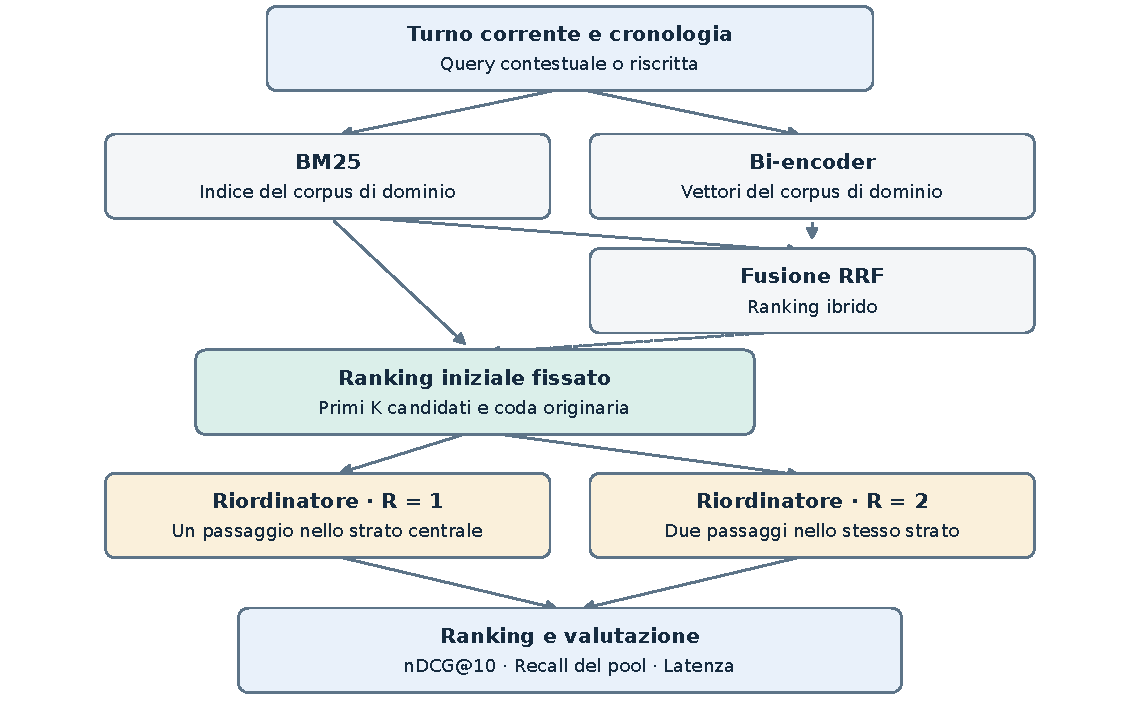
\includegraphics[width=\linewidth]{metodologia_2a.pdf}
 \caption{Flusso del 2a. I canali lessicale e denso producono i ranking del primo stadio. Il confronto principale congela il ranking BM25 contestuale e confronta i riordinatori sui medesimi primi $K$ candidati. La freccia tratteggiata indica l’uso del ranking ibrido come secondo pool, fissato per tutti i bracci del relativo confronto.}
 \label{fig:metodo-2a}
\end{figure}

\paragraph{Adattamento del bi-encoder.}
Adattiamo il bi-encoder con LoRA (rango 16, $\alpha=32$, dropout 0,05) \cite{lora}. Per ogni turno selezioniamo un passaggio positivo tra quelli annotati. Il positivo compete con due negativi difficili campionati da una riserva fino a 40 risultati BM25 e con i positivi associati agli altri esempi del minibatch. La riserva è ricavata dalla query contestuale escludendo i passaggi annotati come pertinenti per quel turno. Nel modo alternato, l'indice dell'esempio e la parità dell'epoca determinano quale formulazione della query si usa. Ogni esempio usa una sola formulazione per epoca e passa all'altra nell'epoca successiva, quando entrambe sono disponibili.

Sia $x_i$ la query effettivamente usata dall'esempio $i$, $p_i$ il suo passaggio positivo e $N_i$ la lista delle posizioni negative. Il contributo dell'esempio alla perdita è
\begin{equation}
 \ell_i=-\log
 \frac{\exp(s(x_i,p_i)/\tau)}
 {\exp(s(x_i,p_i)/\tau)+\sum_{v\in N_i}\exp(s(x_i,d_v)/\tau)},
 \qquad \tau=0{,}05.
 \label{eq:metodo-contrastiva}
\end{equation}
Qui $s$ è la similarità coseno e $d_v$ è il documento nella posizione negativa $v$. Il profilo usa minibatch da quattro esempi, accumulo su due minibatch e un tasso di apprendimento di riferimento di $3\cdot10^{-5}$ preceduto da riscaldamento. I risultati preliminari descrivono il checkpoint della prima epoca documentata.

\paragraph{Fusione dei ranking.}
Consideriamo i ranking lessicale e denso per ciascuna formulazione della query e le loro fusioni. La Reciprocal Rank Fusion assegna a un documento $u$ il punteggio
\begin{equation}
 S_{\mathrm{RRF}}(u)=
 \sum_{m:\,u\in\mathcal L_m}\frac{1}{60+\operatorname{rank}_{\mathcal L_m}(u)},
 \label{eq:metodo-rrf}
\end{equation}
dove $\mathcal L_m$ è la lista del sistema $m$ e il rango parte da uno \cite{rrf}. La fusione usa solo l'ordine delle liste e consente di combinare BM25 e similarità coseno senza confrontarne i punteggi grezzi. Valutiamo anche la fusione mista tra il ranking denso sulla riscrittura e il ranking BM25 sulla query contestuale.

\paragraph{Riordinamento a candidati fissati.}
Per ogni turno fissiamo una lista iniziale e ne prendiamo i primi $K$ documenti. Il protocollo principale usa $K=100$ e una lista BM25 contestuale fino a 1\,000 elementi. Per valutare il loop su candidati ibridi si fornisce allo stesso valutatore un'unica run TREC per tutti i valori di $R$. Il riordinatore Qwen3-Reranker-0.6B riceve un'istruzione di pertinenza, la query contestuale e un documento alla volta come unità logica di valutazione. Il punteggio della coppia è la differenza $z_{\mathrm{yes}}-z_{\mathrm{no}}$ tra i logit dei due token di giudizio \cite{qwen}. Si ordinano i primi $K$ documenti per punteggio decrescente, preservando l'ordine iniziale delle coppie a pari punteggio e accodando la coda originaria.

I due riordinatori ricevono gli stessi candidati nella stessa sequenza e usano lo stesso template e gli stessi limiti di lunghezza. L'impronta SHA-256 dei candidati ordinati per turno verifica il pool in ingresso. Il Recall@$K$ rispetto a $G_t$ quantifica la quota di passaggi pertinenti accessibile al riordinatore. Il contrasto tra $R=1$ e $R=2$ sulla nDCG@10 misura l'effetto del nuovo ordine a parità di pool. La lista originale serve come ulteriore riferimento per quantificare l'effetto complessivo del riordinamento.

\subsection{Subtrack 2b. Dalle evidenze fornite alla risposta}
\paragraph{Costruzione dell'input.}
Per ogni turno recuperiamo dal corpus il testo associato agli identificativi dei passaggi forniti dagli organizzatori. Il prompt contiene istruzioni, domanda, fino a cinque turni di storia e il testo dei passaggi. Nel profilo T4 il limite di input è di 2\,048 token. Dopo aver riservato spazio alle istruzioni e alla domanda, il costruttore limita la storia e assegna alle evidenze il budget residuo. La strategia adattiva ripartisce i token tra i passaggi e li tronca, cercando di conservarne il maggior numero possibile. La Figura~\ref{fig:metodo-2b} distingue il percorso supervisionato, in cui entra la risposta di riferimento, dal percorso di generazione usato nella valutazione.

\begin{figure}[htbp]
 \centering
 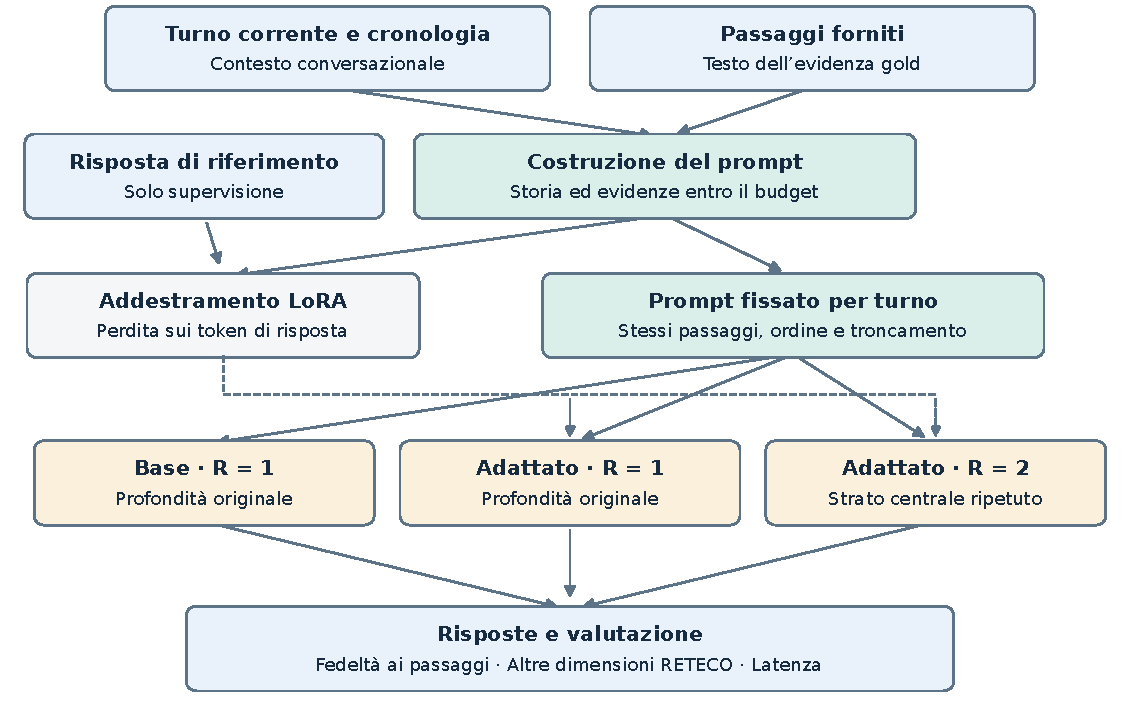
\includegraphics[width=\linewidth]{metodologia_2b.pdf}
 \caption{Flusso del 2b. Il testo dei passaggi forniti dagli organizzatori alimenta il prompt. In addestramento la risposta di riferimento supervisiona i token di uscita. In inferenza lo stesso prompt per turno entra nei bracci a diversa profondità, e le risposte vengono valutate rispetto alle evidenze disponibili. Le frecce tratteggiate indicano il riuso dello stesso adattatore.}
 \label{fig:metodo-2b}
\end{figure}

\paragraph{Adattamento supervisionato.}
Il profilo T4 usa Qwen3-4B-Instruct-2507 con pesi di base quantizzati a 4 bit in formato NF4, calcolo FP16 e adattatori LoRA sulle proiezioni \emph{query} e \emph{value} \cite{lora,qlora}. La configurazione prevede un'epoca, rango 16, $\alpha=32$, dropout 0,05, tasso di apprendimento di riferimento $2\cdot10^{-4}$ e accumulo su otto esempi. L'input di addestramento concatena il prompt $x_t$ alla risposta di riferimento $a_t$. La perdita autoregressiva maschera le posizioni del prompt e del padding:
\begin{equation}
 \ell_t=-\frac{1}{|\mathcal A_t|}\sum_{u\in\mathcal A_t}
 \log p_\theta(a_{t,u}\mid x_t,a_{t,<u}),
 \label{eq:metodo-generazione}
\end{equation}
dove $\mathcal A_t$ contiene le posizioni supervisionate della risposta e $\theta$ indica i parametri del generatore con adattatore. L'equazione esprime la perdita media per un turno, mentre l'implementazione aggrega i token validi del minibatch. In inferenza il prompt termina prima della risposta e il generatore la produce autoregressivamente.

\paragraph{Confronti appaiati.}
Il protocollo prevede tre condizioni sullo stesso insieme di turni: modello base a $R=1$, modello adattato a $R=1$ e stesso modello adattato a $R=2$. Il primo contrasto misura l'effetto dell'adattamento a profondità originale. Il secondo misura l'effetto della profondità a checkpoint fissato. Congeliamo testo, ordine e troncamento dei passaggi, template, cronologia e parametri di generazione. Usiamo decodifica greedy diretta, una risposta per turno, un massimo di 256 nuovi token e penalità di ripetizione 1,05. La fedeltà alle evidenze è la dimensione primaria proposta. Correttezza, completezza, pertinenza e coerenza conversazionale descrivono gli altri aspetti della risposta secondo la rubrica RETECO \cite{evaluation}. Registriamo anche la lunghezza generata e la latenza per risposta, così da interpretare il costo a fronte sia del numero di applicazioni di strato sia del numero di token prodotti.

\section{Risultati preliminari}
\subsection{Validazione del primo stadio di recupero}
Alla fine della prima epoca, dopo 450 minibatch, la perdita media è 0,9766 (deviazione standard tra minibatch 0,6671). La frazione di positivi al primo posto tra i candidati di addestramento è 0,6328. Il tempo registrato per l'epoca è 3\,583 secondi. Valutare il ranking sull'intero corpus richiede il calcolo degli embedding di ciascuna collezione: per Earth Science, ad esempio, trascorrono circa 129 minuti dall'avvio della validazione di dominio alla disponibilità dei 121\,249 vettori. Il tempo dell'epoca da solo sottostima quindi il costo dell'esperimento.

La Tabella~\ref{tab:domains} riporta tutti i domini per i quali il log del 25 novembre documenta il completamento. Per Sustainable Living il log termina durante la codifica dei documenti; i suoi 32 turni restano fuori dal denominatore. Per ogni dominio calcoliamo la media di nDCG@10 sui turni; l'ultima riga assegna uguale peso ai dieci domini osservati. I valori derivano dai punteggi di dominio arrotondati a quattro decimali.
\begin{table}[htbp]\centering\small
\caption{nDCG@10 di validazione interna nell'epoca 1 del 2a. C indica la query contestuale, S la riscrittura. La fusione mista usa il denso S e BM25 C. I due gruppi di domini corrispondono a BRIGHT e StackExchange.}\label{tab:domains}
\setlength{\tabcolsep}{3pt}
\begin{tabular}{lr rr rr rrr}\toprule
& & \multicolumn{2}{c}{Denso} & \multicolumn{2}{c}{BM25} & \multicolumn{3}{c}{RRF}\\
\cmidrule(lr){3-4}\cmidrule(lr){5-6}\cmidrule(lr){7-9}
Dominio & Turni & C & S & C & S & C & S & Mista\\\midrule
Biology & 33 & 0.0689 & 0.0598 & 0.5649 & 0.4264 & 0.5329 & 0.4390 & 0.5142 \\
Earth Science & 46 & 0.1905 & 0.1702 & 0.6465 & 0.5940 & 0.6021 & 0.5363 & 0.6179 \\
Economics & 28 & 0.0376 & 0.0421 & 0.4041 & 0.4418 & 0.3279 & 0.3162 & 0.3171 \\
Psychology & 43 & 0.1792 & 0.1166 & 0.7077 & 0.5493 & 0.6701 & 0.5343 & 0.6497 \\
Robotics & 26 & 0.0904 & 0.0389 & 0.3652 & 0.3174 & 0.5197 & 0.4034 & 0.4665 \\
\midrule
Drones & 17 & 0.6197 & 0.6186 & 0.3342 & 0.3072 & 0.7473 & 0.6999 & 0.7582 \\
Hardware & 22 & 0.3229 & 0.3385 & 0.2377 & 0.1705 & 0.5987 & 0.5674 & 0.6234 \\
Law & 25 & 0.7169 & 0.7146 & 0.2818 & 0.1668 & 0.6890 & 0.5439 & 0.6902 \\
Medical Sciences & 21 & 0.7196 & 0.5936 & 0.1892 & 0.1310 & 0.7188 & 0.5070 & 0.6888 \\
Politics & 19 & 0.8555 & 0.7638 & 0.4361 & 0.3561 & 0.8352 & 0.7877 & 0.7885 \\
\midrule
Media macro & 280 & 0.3801 & 0.3457 & 0.4167 & 0.3461 & 0.6242 & 0.5335 & 0.6114 \\\bottomrule\end{tabular}\end{table}

La fusione contestuale raggiunge 0,6242 contro 0,4167 per BM25 e 0,3801 per il denso. La differenza rispetto a BM25 è particolarmente ampia in Drones (0,7473 contro 0,3342). In Biology, invece, BM25 supera la fusione (0,5649 contro 0,5329). Anche quando il denso individua un documento pertinente nella lista estesa, può collocarlo troppo in basso: in Biology il suo Recall@1000 è 0,9343, mentre il Recall@10 scende a 0,1439. Per i candidati di un riordinatore con $K=100$ il valore pertinente è Recall@100, qui pari a 0,5985 per il denso e 0,8434 per BM25.
\begin{figure}[htbp]\centering
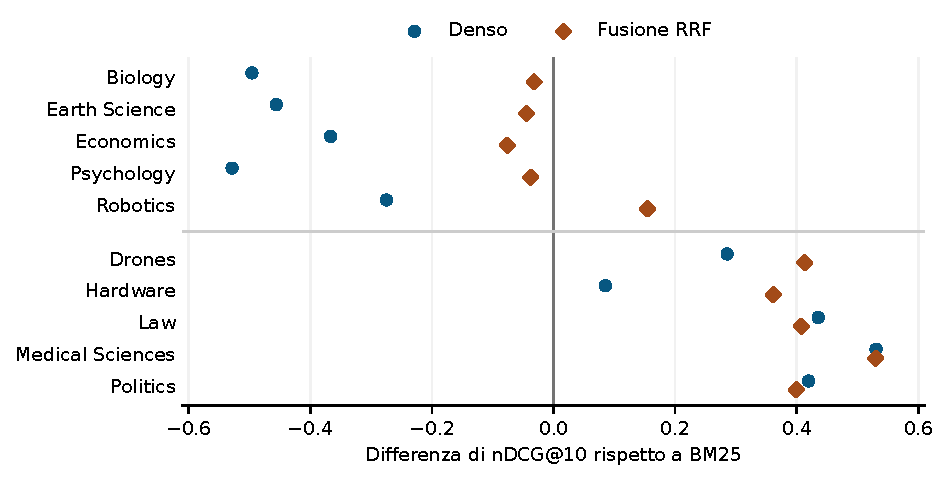
\includegraphics[width=.87\linewidth]{confronto_per_dominio.pdf}
\caption{Differenze rispetto a BM25 con la stessa query contestuale. A destra dello zero il sistema supera BM25. La linea orizzontale separa le due origini delle collezioni. Ogni punto è una differenza tra medie sullo stesso insieme di turni.}\label{fig:domains}
\end{figure}

\subsection{Misure previste per il confronto di profondità}
Per il 2a il confronto primario sarà $R=2$ contro $R=1$ sugli stessi candidati; $R=4$ servirà come analisi esplorativa di sensibilità. Per un dominio $d$, indichiamo con $m_{t,R}$ la nDCG@10 del turno $t$ alla profondità $R$. L'effetto principale sul dev sarà
\[
 \Delta_{2a}=\frac1{11}\sum_{d=1}^{11}\frac1{n_d}\sum_{t\in d}
 (m_{t,2}-m_{t,1}).
\]
Registreremo la copertura dei candidati prima del riordinamento, la latenza per query senza riuso dei punteggi e la memoria GPU di picco. Per quantificare l'incertezza prevediamo un bootstrap appaiato stratificato per dominio, ricampionando intere conversazioni e mantenendo insieme i loro turni. Gli intervalli al 95\% descriveranno la variabilità campionaria a checkpoint fissato.

Nel 2b il criterio primario proposto è la fedeltà ai passaggi; correttezza, completezza, pertinenza e coerenza conversazionale completano il profilo. Adotteremo la scala intera 1--5 per ciascuna dimensione e la trasformazione $(s-1)/4$ del protocollo RETECO \cite{evaluation}. Per una valutazione locale cieca, le risposte saranno anonimizzate e presentate in ordine casuale con domanda, storia ed evidenze identiche; conserveremo anche casi di parità e risposte mancanti. Prevediamo un secondo giudizio indipendente su un sottoinsieme per verificare l'accordo. Riporteremo le differenze appaiate, i token prodotti e i secondi per risposta. I log disponibili documentano il primo stadio del 2a; nessuna misura comparativa di profondità o di qualità delle risposte 2b è ancora disponibile.

\section{Discussione}
\paragraph{La scelta dei candidati dipende dalla collezione.}
La Figura~\ref{fig:domains} mostra una regolarità che la media nasconde. Il denso contestuale supera BM25 in ciascuno dei cinque domini di origine StackExchange; BM25 prevale in ciascuno dei cinque domini BRIGHT con dati disponibili. Questa suddivisione segue la provenienza documentata dagli organizzatori \cite{data}. Dimensione delle collezioni, numero di passaggi pertinenti e formulazione delle domande variano insieme alla provenienza. I dati consentono di descrivere l'associazione; attribuirla a una singola proprietà richiederebbe controlli ulteriori. In Robotics, dove il denso ottiene appena 0,0904, la sua fusione con BM25 raggiunge comunque 0,5197. Un retriever debole preso isolatamente può dunque contribuire al primo stadio ibrido. La scelta di un pool congelato è essenziale per stabilire quanto possa aggiungere il riordinamento.

\paragraph{Cosa confrontare con i riferimenti degli organizzatori.}
Per il 2a gli organizzatori pubblicano sul dev completo una nDCG@10 macro di 0,1827 per BM25 sul solo turno e di 0,4379 includendo la storia \cite{data}. La nostra Tabella~\ref{tab:domains} usa una partizione interna di train, copertura parziale dei domini e un'implementazione BM25 nativa Lucene. Una differenza numerica tra le due tabelle confonderebbe sistema e partizione. Il confronto esterno richiede una run su tutti gli 858 turni dev, valutata con gli stessi giudizi e la stessa aggregazione. Un eventuale piazzamento nella classifica del test nascosto richiederà il risultato ufficiale della submission. Per il 2b gli organizzatori pubblicano cinque giudizi distinti a fianco del recupero \cite{evaluation}; un giudizio locale dovrà riportare valutatore e rubrica e mantenere esplicita la sua provenienza.

\paragraph{Quale risultato giustificherebbe il loop?}
Per il 2a una differenza positiva su candidati identici indicherebbe una migliore disposizione delle evidenze accessibili. Esaminare i turni in cui un passaggio entra o esce dalle prime dieci posizioni aiuterebbe a capire se il cambiamento riguarda riferimenti al dialogo o semplici corrispondenze lessicali. Per il 2b una risposta può diventare più completa introducendo un dettaglio privo di sostegno: leggere separatamente completezza e fedeltà evita di perdere questa informazione in un unico punteggio. Un beneficio circoscritto a uno dei compiti sarebbe interpretabile, poiché decidere tra due logit e produrre una sequenza autoregressiva impongono vincoli diversi. A qualità simile, il decoder originale offre il riferimento per giudicare il costo di ogni passaggio ulteriore.

\paragraph{Limiti e riproducibilità.}
I risultati disponibili riguardano un seme, un checkpoint e dieci domini. I soli aggregati di console non permettono di ricostruire intervalli appaiati per conversazione. Per le misure finali occorrerà conservare ranking e risposte per turno, configurazioni effettive, revisioni di codice e pesi, impronte dei candidati, modello di GPU e precisione effettiva. Il profilo destinato a T4 è un vincolo di progetto; i tempi sopra riportati descrivono il singolo log. Il codice del progetto è disponibile all'indirizzo \url{https://github.com/GiovanniIacuzzo/SemEval-2027-Task-1}; la metodologia qui descritta si riferisce alla revisione locale con il loop per entrambi i subtrack.

\section{Conclusioni}
Nel recupero conversazionale di RETECO, la scelta di come costruire la lista dei candidati incide già prima di introdurre calcolo aggiuntivo nel decoder. Nella validazione interna disponibile la fusione contestuale ottiene la migliore media tra le sette configurazioni esaminate, pur cedendo a un singolo retriever in diversi domini. Questo risultato individua due condizioni sperimentali informative: un pool lessicale riproducibile e un pool ibrido più competitivo in media.

L'implementazione consente ora di porre la stessa domanda sulla profondità in due condizioni distinte: riordinare evidenze già reperite oppure formulare una risposta a partire da evidenze fornite. Il passo decisivo per il preprint è misurare, a turno e input fissati, la differenza rispetto a una sola applicazione dello strato, insieme al tempo necessario per ottenerla. Da quel confronto dipenderà la conclusione sull'utilità della ricorrenza.


\bibliographystyle{plain}
\bibliography{references}
\end{document}
